\documentclass[12pt,letterpaper]{article}
\input{../../preamble}
\usepackage{fullpage}
\usepackage{multicol}

\begin{document}
\flushleft
\begin{multicols}{2}
\textbf{Math 2554 Exam 3: $\oint 3.8-4.5$ \\
Friday 3 April 2015}

%\hfill
\textbf{Name:  }\underline{\hspace{45ex}} %KEY\hspace{17ex}}

\vspace{.5in}

\end{multicols}

\pagestyle{empty}

\flushleft

\begin{center}\LARGE Calculus I 

Exam 3: The Story Problem Exam \end{center}

\vspace{1.5pc}
Please provide the following data:

\vspace{1.5pc}
Drill Instructor: \underline{\hspace{40ex}}

\vspace{1.5pc}
Drill Time: \underline{\hspace{40ex}}

\vspace{1.5pc}
Student ID or clicker \#: \underline{\hspace{40ex}}

%\vfill
\vspace{3pc}
{\bf Exam Instructions:} You have 50 minutes to complete this exam.  One $3\times 5$ inch notecard, one side only, is allowed.  No graphing calculators.  No programmable calculators.  No electronic devices except for the approved calculators (so no phones, iDevices, computers, etc).  If you finish early then you may leave, UNLESS there are less than 5 minutes of class left.  To prevent disruption, if you finish with less than 5 minutes of class remaining then please stay seated and quiet.

%\vspace{2pc}
\vfill
\textbf{Your signature below indicates that you have read this page and agree to follow the Academic Honesty Policies of the University of Arkansas.}  

\vspace{2pc}
Signature: {\bf (1 pt)} \underline{\hspace{91ex}}

%\vfill
\begin{flushright}\Large Good luck!\end{flushright}

% % % % %	
\newpage

\begin{enumerate}[1.]

\item {\bf (3 pts ea)} Let $g(x)=\ln{(1+x)}$.
	\begin{enumerate}
	\item Write the equation for the linear approximation to $g(x)$ at $x=0$.
	
	\vspace{12pc}
	\item Use your answer to (a) to approximate $g(0.9)$.

	\vspace{6pc}
	\item Below is the graph of $g(x)$, drawn at the website \url{desmos.com/calculator}. On the same axis, draw your tangent line.  Label both $g(0.9)$ and your approximation from part (b).
	
	\vspace{2pc}
	\centering{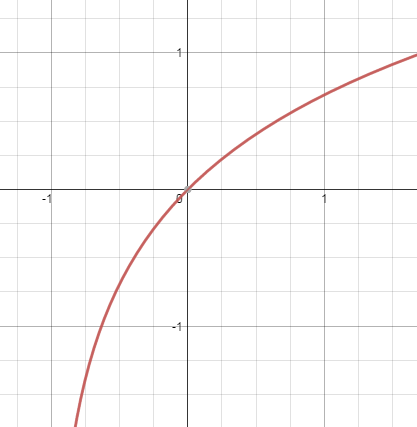
\includegraphics[scale=0.85]{exam3pic1c}}
	\end{enumerate}
	
% % %
\newpage
\item {\bf (13 points)} Your boss keeps cookies on the top shelf there but there is a hole in the bag.  The cookies are spilling, accumulating in a cone-shaped pile whose radius ($r$) is always three times the cone's height ($h$).  Your boss won't eat the cookies once they fall out of the bag.  If the height of the pile is increasing at a rate of $2$ cm/s when the pile is $12$ cm high, how fast is your boss losing his eat-able cookies in that instant?  

\vspace{1pc}The volume of the cone is $V=\frac{1}{3}\pi r^2h$.  Round your final answer to one decimal place (if you try to tell your boss a number with $\pi$ in it, he will likely get confused and angry!).

% % %
\newpage
%\vspace{26pc}
\item {\bf (2 pts ea)} Evaluate.  You do not need to simplify your answers. {\it Hint: In some of these problems it is quicker if you remember the properties of logs.} 

	\begin{enumerate}
	\item $\displaystyle \dfrac{d}{dy}\log_2{\frac{8}{\sqrt{y+1}}}$
		
	%\vspace{15pc}
	%\newpage
	%\item $\displaystyle \dfrac{d}{dz}\ln{\frac{2z}{(z^2+1)^3}}$
	
	%\vspace{15pc}
	%\item $\displaystyle \dfrac{d}{dw}\sin{\left(\sec^{-1}(2w)\right)}$
	
	\vspace{15pc}
	%\newpage
	\item $\displaystyle \dfrac{d}{du}\tan^{-1}\left(e^{4u}\right)$
	
	\vspace{15pc}
	%\newpage
	\item $\displaystyle \dfrac{d^n}{dx^n}2^x$ \hspace{3ex}($n$ is a positive integer)
	
	%\vspace{15pc}
	%\newpage
	%\item $\displaystyle \dfrac{d}{dv}\cot^{-1}\left(\frac{1}{v^2+1}\right)$
	\end{enumerate}
	
% % %
\newpage
%\vspace{15pc}
\item The goal of this problem is to produce a graph of the function
%\[f(x)=\frac{1}{e^{-x}-1}\]
\[f(x)=xe^{-x}\]
from scratch.
	
	\begin{enumerate}
	\item {\bf (2 pts)} Find the domain for $f(x)$.
	
	\vspace{8pc}
	\item {\bf (2pts)} Is $f(x)$ even, odd, or neither?  You must justify your answer.
	
	\vspace{10pc}
	\item {\bf (4 pts)} Find $f'(x)$ and $f''(x)$.  You are not required to simplify.
	
	% %
	\newpage
	%\vspace{10pc}
	\item {\bf (3 pts)} Find the critical points.  If there are none, then say why.
	
	% %
	%\newpage
	\vspace{14pc}
	\item {\bf (3 pts)} Find the possible inflection points.  If there are none, then say why.
	
	\vspace{14pc}
	\item {\bf (3 pts)} What are the intervals where $f(x)$ is increasing?  What are the intervals where $f(x)$ is decreasing?
	
	% %
	\newpage
	%\vspace{10pc}
	\item {\bf (3 pts)} What are the intervals where $f(x)$ is concave up?  What are the intervals where $f(x)$ is concave down?
	
	% %
	%\newpage
	\vspace{23pc}
	\item {\bf (4 pts)} Find the local extrema and inflection points.  You must justify your answers.  If there are no extrema or inflection points you should also say why.
	
	% %
	\newpage
	%\vspace{12pc}
	\item {\bf (2 pts)} Find the vertical asymptotes, using the limit definition of a vertical asymptote.  If there are no vertical asymptotes, then say so.
	
	\vspace{14pc}
	\item {\bf (2 pts)} Determine the end behavior.  
	
	{\it Hint: By L'\^opital's Rule ($\oint 4.7$), 
	\[\displaystyle\lim_{x\to\infty}xe^{-x}=\lim_{x\to\infty}\frac{1}{e^x}.\]  
	For $\displaystyle\lim_{x\to -\infty}f(x)$ you do not need L'\^opital's Rule.} 
	
	% %
	\newpage
	%\vspace{20pc}
	\item {\bf (2 pts)} Find the $y$-intercepts and $x$-intercepts, if there are any.  
	
	% %
	%\newpage
	\vspace{18pc}
	\item {\bf (3 pts)} Using all the information above, draw a well-labeled graph of $f(x)$.  Your picture should be consistent with your answers to (a)-(k).
	\end{enumerate}
	
% % % 
\newpage
\item {\bf (13 points)} A rectangle is constructed with its base on the $x$-axis and two of its corners on the parabola $y=16-4x^2$.  What are the dimensions of the rectangle with the maximum area?  {\it Hint: The picture of the parabola is given (using \url{desmos.com/calculator}).}

\vspace{2pc}
%\begin{flushright}
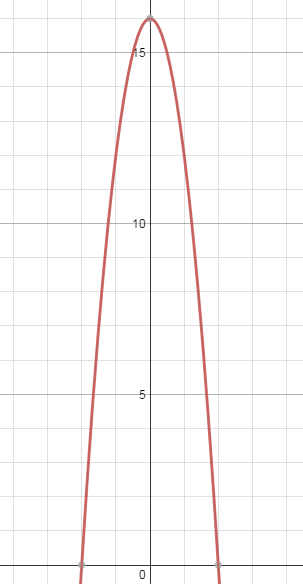
\includegraphics[scale=0.75]{exam3pic5}%\hspace{50ex}  \end{flushright}

%{\bf You do not need to simplify your final answer in this problem.}  An isoceles triangle is a triangle where two sides are equal (the third side may or may not be equal to the others).  The radius $r$ of a circle inscribed in any triangle is given by the formula
%\[r=\frac{2A}{P},\]
%where $A$ is the area of the triangle and $P$ is the perimeter of the triangle.

%\vspace{1pc}
%What is the radius of the biggest circle that can be inscribed in an isoceles triangle whose two equal sides have length 1?  {\it Hints: Use the Pythagorean Theorem to get the height of the triangle.  If possible, simply the objective function.  If the derivative is too nasty, logarithmic differentiation might be quicker.}  

% % %
\newpage
\vspace{20pc}
\item {\bf ChAlLeNgE pRoBlEm (0 pts)} Using the graphs of $f'$ and $f''$, draw a possible graph for $f(x)$ on the same axes, assuming $f(0)=0$.  {\it Hint: Use the picture to find intervals where $f$ is increasing/decreasing, concave up/down, critical points, inflection points, etc.} 

\vspace{2pc}
\centering{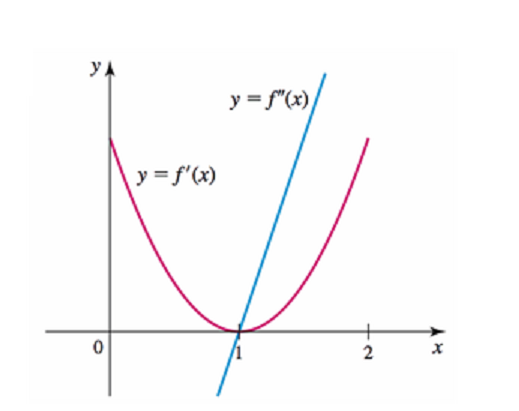
\includegraphics[scale=1.1]{exam3picCP}

{\footnotesize taken from {\it Calculus: Early Transcendentals}, Briggs et al.}
}
\end{enumerate}

\end{document}